\chapter{Experiments and analyses}
\label{cap:experiments}

In this chapter the experiments leading to the proposed solution of this thesis are presented.

First, the evaluation methodology is presented in \Cref{sec:exp_evaluation}.
Then, the four implemented reference models are benchmarked in \Cref{sec:exp_reference_benchmark}, followed by experimental analysis with the aim of improving the effectiveness of the best reference model in \Cref{sec:exp_improving_tcn}.
Once it became clear that the reference model and its variants improved with diminishing returns on the test split, I changed direction.
The new aim was to reduce parameter count and computational delay while keeping macro F1 score comparable with the reference TCN.
This is presented in \Cref{sec:exp_lightweight}.
Finally, the proposed models are analyzed in comparison to the references in \Cref{sec:exp_analyses}.

\section{Evaluation methodology}
\label{sec:exp_evaluation}

This section describes the frame-level evaluation procedure, the motivation behind the F1 metrics used, and the significance test applied to every classifier.

\subsection{Frame-level evaluation}
\label{subsec:exp_eval_frame}

The on-line constraints (\Cref{subsec:constraints}) require every classifier to operate at \textbf{frame level}, with the output rate matching each model's frame hop (TCN $23.2\,\text{ms}$, GMM and SVM $15\,\text{ms}$, decision tree $10\,\text{ms}$).
Each output prediction is compared against a per-frame ground-truth label.
Each frame is labeled with the class that holds the largest share of its duration in the dataset's timestamped intervals (\Cref{sec:dataset_labeling}).

\subsection{Metrics}
\label{subsec:exp_eval_metrics}

For each class $c \in \{\text{\emph{Speech}}, \text{\emph{Music}}, \text{\emph{Background}}\}$, let $\mathrm{TP}_c$, $\mathrm{FP}_c$, and $\mathrm{FN}_c$ denote the number of true positive, false positive, and false negative frames over the evaluation split, computed one-vs-rest.
Precision and recall for class $c$ are
\begin{align}
\label{eq:precision_recall}
P_c &= \frac{\mathrm{TP}_c}{\mathrm{TP}_c + \mathrm{FP}_c}, &
R_c &= \frac{\mathrm{TP}_c}{\mathrm{TP}_c + \mathrm{FN}_c},
\end{align}
and the \textbf{per-class F1} is their harmonic mean:
\begin{align}
\label{eq:f1_class}
F1_c &= \frac{2\, P_c \cdot R_c}{P_c + R_c} = \frac{2\, \mathrm{TP}_c}{2\, \mathrm{TP}_c + \mathrm{FP}_c + \mathrm{FN}_c}.
\end{align}
F1 weights false positives and false negatives equally, so a model cannot trade one for the other to inflate the score.

The \textbf{macro F1 score} is the unweighted mean of the three per-class F1s:
\begin{align}
\label{eq:macro_f1}
\text{macro }F1 &= \frac{1}{3} \sum_{c} F1_c.
\end{align}
Averaging the per-class F1 gives every class equal weight regardless of frame count, so smaller classes contribute as much to the final score as larger ones.
The macro F1 score is the headline metric for every experiment in this chapter.

Per-class F1 shows the contribution of each class to the macro F1 score.

Each reported macro F1 score is accompanied by a $95\,\%$ \textbf{confidence interval (CI)}: a band around the score that captures how much it could plausibly have shifted with a different mix of clips in the test split.
The CI was added in response to a problem encountered in the first three experiments of \Cref{sec:exp_improving_tcn} (\Cref{subsec:exp_sensitivity,subsec:exp_frontend,subsec:exp_preprocessor}): many variants' macro F1 scores landed within a few thousandths of the reference TCN, and a $+0.003$ gain could equally reflect a real improvement or just noise from the specific clips in the test split.
The scores alone offered no way to tell.

The CI is constructed by a \textbf{cluster bootstrap}~\cite{efron1979bootstrap,davison1997bootstrap}: clips, not individual frames, are the unit of resampling because frames within one clip share speaker, recording conditions, and buffer state.
Frame-level resampling would treat each frame as an independent measurement and shrink the CI artificially.
$1\,000$ alternative ``test splits'' are built by drawing clips from the actual test split at random with replacement, each one the same clip count as the original but with a different mix: each draw is independent, so the same clip can appear multiple times in a resample and roughly $37\,\%$ of the original clips are absent from it.
The macro F1 score is recomputed on each, producing a distribution of $1\,000$ alternative scores around the actual test-split score.
The CI is the range from the $2.5$th to the $97.5$th percentile of this distribution.

CIs are read as a guide rather than a strict cutoff.
A CI that cleanly separates from the reference's is taken as strong evidence of a real difference.
Overlapping CIs are read more cautiously: the gap may still reflect a real effect, but the test split does not settle the question on its own.

The CI captures test-split variability only.
Training itself is non-deterministic, since random weight initialization, data shuffling, and parallel arithmetic produce slightly different checkpoints from the same recipe on each run.
A fixed random seed is used for every variant in this thesis to hold this second source of variance constant, and a multi-seed reproduction that would also capture training variance is listed as future work in \Cref{sec:conclusion_future}.

\section{Benchmark on reference models}
\label{sec:exp_reference_benchmark}

The four reference classifiers are benchmarked on the test split (\Cref{sec:dataset_subsets}).
The strongest of them will be the focus of the experiments that follow.
\Cref{fig:reference_benchmark} presents the results.
DT abbreviates the decision tree in plots and tables.

\begin{figure}[h]
\centering

\includegraphics[width=0.75\textwidth]{figures/experiments/reference_benchmark.pdf}
\caption{Per-class F1 (bars) and macro F1 score ($\diamond$) benchmark results.}
\label{fig:reference_benchmark}
\end{figure}


The TCN wins.
It sits roughly $0.10$ macro F1 score above the strongest traditional model.
Its lead holds across all three classes.

The three traditional references cluster between $0.825$ and $0.875$ macro F1 score, while the TCN reaches $0.975$, roughly twice that cluster width above the strongest traditional model.
The ranking therefore does not depend on which traditional model is taken as the comparison reference.

The causal TCN is selected as the experimental focus for the rest of the chapter.

\section{Improving the TCN}
\label{sec:exp_improving_tcn}

The reference TCN achieves macro F1 score of $0.9752$ with a CI of $[0.9687, 0.9794]$.
This section asks whether further improvements are available.
The TCN is analyzed first, then five experiments replace or add to its components.

\subsection{Sensitivity analysis and ablation}
\label{subsec:exp_sensitivity}

The reference configuration is summarized in \Cref{tab:reference_config}.

\begin{table}[h]
\centering
\small
\begin{tabular}{l l @{\hskip 2em} l l}
\toprule
\multicolumn{2}{l}{\textbf{Architecture}} & \multicolumn{2}{l}{\textbf{Optimization}} \\
\addlinespace
filters          & $16$         & optimizer     & SGD, momentum $0.9$ \\
layers per stack & $4$          & learning rate & $10^{-3}$ \\
stacks           & $3$          & batch size    & $32$ \\
kernel size      & $5$          & loss          & BCE-with-logits \\
\addlinespace
dropout          & $0.5$        & \multicolumn{2}{l}{\textbf{Input}} \\
\addlinespace
normalization    & WeightNorm   & frontend      & $80$-bin log-mel \\
activation       & ReLU         & chunk length  & $128$ frames \\
\bottomrule
\end{tabular}
\caption{Reference TCN configuration.}
\label{tab:reference_config}
\end{table}

Each experimental variant changes exactly one of these parameters, retrains for $50$ epochs on the full subset with early-stopping patience of $5$ epochs, and is compared against the reference TCN.
The variants split into two groups:
\begin{enumerate}
    \item \textbf{Structural and categorical variation} either removes a component (ablation) or swaps a discrete choice along one of four categorical dimensions: optimizer, normalization, activation, or loss.
    \item \textbf{Hyperparameter sensitivity} varies a numerical parameter (learning rate, dropout, layer count, filter count, kernel size, sequence length, batch size).
\end{enumerate}
Several groups landed within $\pm 0.003$ of the reference.
Those are pruned from the active configuration and listed at the end of this section.

\subsubsection{Structural and categorical variation}
\label{subsubsec:exp_substitution}

The only structural ablation tested removes the residual (skip) connections in every TCN block.
Without them, macro F1 score collapses to $0.1884$: the model predicts \emph{Music} for every frame, with \emph{Speech} and \emph{Background} recalls both $0$.
The residual connections are therefore essential.

The substitution scan swaps each of three categorical choices in the reference TCN (optimizer, normalization, activation) for an alternative.
\Cref{fig:sensitivity_substitution} reports the result.
The same plot style is reused for every variant scan in the rest of \Cref{sec:exp_improving_tcn}: bars show macro F1 score with CI whiskers, and the gray band marks the reference CI.

\begin{figure}[h]
\centering

\includegraphics[width=\textwidth]{figures/experiments/sensitivity_substitution.pdf}
\caption{Component substitution scan.}
\label{fig:sensitivity_substitution}
\end{figure}

The optimizer category pairs Adam~\cite{kingma2015adam} with BatchNorm~\cite{ioffe2015batchnorm}.
Bare Adam was tested separately and diverged to a trivial speech-only predictor (not shown).
The normalization category swaps WeightNorm for BatchNorm under SGD, which is neutral.

The activation category shows no significant change for GeLU or LeakyReLU.
ELU is the only activation with a noticeable difference, and even that is only $-0.0113$.

Every substitution variant's CI overlaps the reference TCN, so no shift in this scan is strict under the CI rule defined in \Cref{subsec:exp_eval_metrics}.
The loss family (focal, class-weighted BCE, MSE, label-smoothed BCE) is similarly flat at $\pm 0.0003$ of the reference and is not plotted.

\subsubsection{Hyperparameter sensitivity}
\label{subsubsec:exp_hyperparam}

The sensitivity scan shifts three numerical parameters (learning rate, dropout, and layer count) along the ranges described in the reference paper~\cite{lemaire2019tcn}.

Like the substitution scan, this one produces no strict gains.
Tested values and their macro F1 score are shown in \Cref{fig:sensitivity_hyperparam}.

Lowering dropout and raising the learning rate both increase macro F1 score by a margin comparable to the Adam+BatchNorm substitution in the previous figure.

The TCN variant with only one layer is the only one in this sensitivity scan whose CI separates from the reference TCN.
Its receptive field collapses to $25$ frames ($\approx 580\,\text{ms}$), well below any other configuration in this thesis.
The two- and three-layer variants stay inside sampling noise.

\begin{figure}[h]
\centering

\includegraphics[width=\textwidth]{figures/experiments/sensitivity_hyperparam.pdf}
\caption{Hyperparameter sensitivity scan.}
\label{fig:sensitivity_hyperparam}
\end{figure}

Other numerical hyperparameters were tested but produced flat results across every value (\Cref{tab:sensitivity_pruned}).

\begin{table}[h]
\centering
\begin{tabular}{lll}
\toprule
\textbf{Parameter} & \textbf{Tested values} & \textbf{$\Delta$F1} \\
\midrule
filter count   & $8$, $32$         & $\pm 0.003$ \\
stack count    & $5$               & $\pm 0.001$ \\
kernel size    & $3$, $7$, $9$     & $\pm 0.003$ \\
chunk length   & $256$, $270$      & $\pm 0.002$ \\
batch size     & $16$, $64$        & $\pm 0.002$ \\
\bottomrule
\end{tabular}
\caption{Hyperparameter sensitivity variants whose macro F1 score landed within sampling noise of the reference TCN.}
\label{tab:sensitivity_pruned}
\end{table}


Mel-bin alternatives at $40$ and $128$ bins do not appear here because they are evaluated in the frontend scan of \Cref{subsec:exp_frontend} instead.

\subsubsection{Takeaway}

One-at-a-time changes within the bounds of the original recipe produce small, scattered effects.
Every change landed inside the reference CI or strictly below it.
No variant within Lemaire and Holzapfel's proposed TCN hyperparameter bounds is therefore adopted as a new model.

I have taken the reference TCN as the foundation of the thesis's proposed method.
The following experiments in this section determine its final form.

\subsection{Spectral frontend}
\label{subsec:exp_frontend}

This experiment tries different fixed (non-learned) frontends because different representations of the spectrum may suit the TCN's first layer better than log-mel alone.
Variants cover three families: 
\begin{enumerate}
	\item log-mel bin count: $40$, $80$, $128$
	\item log-mel temporal derivatives: $\Delta$ and $\Delta^2$
	\item energy-normalization alternatives: $20$ and $40$ MFCCs, PCEN
\end{enumerate}

$\Delta$ and $\Delta^2$ are first- and second-order frame-to-frame differences of the log-mel spectrogram~\cite{furui1986dynamic}, concatenated as extra channels alongside the original.
$\Delta$ doubles the channel count to $160$, $\Delta^2$ triples it to $240$.

PCEN (per-channel energy normalization)~\cite{wang2017pcen} replaces the log compression of the log-mel frontend with a per-channel adaptive automatic gain control followed by a soft power-law compression.

\begin{figure}[h]
\centering

\includegraphics[width=\textwidth]{figures/experiments/frontend.pdf}
\caption{Spectral frontend scan.}
\label{fig:frontend_results}
\end{figure}

\break

Results show that frequency resolution is not the discriminative bottleneck.
The mel-bin scan is flat, and MFCC confirms the verdict at one-quarter of the input dimensionality.

The temporal-derivative variants are the largest positive moves across the chapter's scans.
The TCN's first-layer convolution does not extract short-term spectral derivatives as cleanly as a hand-coded delta operator, and pre-computing them gives the backbone cleaner derivative features as input.

PCEN is the only frontend that strictly regresses.
Its automatic-gain-control behavior strips level cues that the log-mel z-normalization already preserves, producing a double-normalization that hurts the \emph{Background} class specifically.
PCEN replacing the log-mel z-normalization rather than adding to it might recover the lost ground.
This was not tested.

The $\Delta^2$ frontend is selected for the combined experiment in \Cref{sec:exp_combined}.

\subsection{Learned preprocessor}
\label{subsec:exp_preprocessor}

This experiment inserts a learned preprocessor between the log-mel frontend and the TCN body to test whether explicit input-side processing before the backbone helps.

Two variants are tested.
A 1-D convolution treats the 80 mel bins as channels and mixes them all at once.
A 2-D convolution treats the spectrogram as an image and mixes only neighboring time-frequency cells through a $3 \times 3$ kernel.
Both variants use a 3-frame causal temporal kernel, so the lookback is identical.

The results are presented in \Cref{fig:preprocessor_results}.
The parenthesized number next to each variant's macro F1 score is a relative parameter count compared to the reference TCN.

\begin{figure}[h]
\centering

\includegraphics[width=\textwidth]{figures/experiments/preprocessor.pdf}
\caption{Learned-preprocessor scan.}
\label{fig:preprocessor_results}
\end{figure}

\break

The 1-D variant's gain is consistent with channel-mixing depth the TCN's $1{\times}1$ input projection cannot provide on its own.
The 2-D variant's dip is consistent with its small spectro-temporal patches duplicating what the backbone's dilated blocks already construct.
Both sit within sampling noise, but the directional gap suggests an architecture-aware preprocessor may help.

The 1-D channel-mixing preprocessor is selected for the combined experiment in \Cref{sec:exp_combined}.

\subsection{Alternative backbones}
\label{subsec:exp_architecture}

This experiment swaps the TCN body for recurrent and attentive alternatives to check whether they fit the task better than the TCN.

Three alternative backbones (GRU, LSTM, Transformer) are tested at two parameter budgets, with the rest of the recipe held constant.
The smaller budget targets $\sim 30$\,K parameters, matching the reference TCN.
The larger budget targets $\sim 130$\,K parameters, matching the TCN scaled to filter count $F=32$, included as a same-family reference.

$F$ denotes each backbone's width parameter.
For GRU and LSTM, $F$ is the hidden state size and for the Transformer, $F$ is the model dimension.

\begin{figure}[h]
\centering

\includegraphics[width=\textwidth]{figures/experiments/architecture.pdf}
\caption{Backbone architecture scan.}
\label{fig:architecture_results}
\end{figure}

\break

The TCN family leads at both budgets by score, but every CI in the recurrent cluster overlaps the reference TCN and the others.
The lead is direction-stable across the small and large tiers but not strict.

The Transformer is the strict outlier of the experiment: both variants land below the reference CI, and the large variant regresses with scale instead of improving.
The large Transformer reaches macro F1 score $0.6942$ (omitted from the plot for scale), with the failure concentrated on the \emph{Background} class (recall $0.20$, F1 $0.32$).
This work does not provide enough training data for the Transformer, though this hypothesis is not investigated further.

No alternative backbone beats the TCN.
The larger TCN at $F=32$ is carried into the next experiment to test capacity increase together with the frontend and preprocessor winners.

\subsection{Combined variants}
\label{sec:exp_combined}

This experiment combines the three best-performing variants from three previous experiments to test whether their individual gains compose.
The selected modifications are F ($\Delta^2$ frontend, \Cref{subsec:exp_frontend}), P (1-D preprocessor, \Cref{subsec:exp_preprocessor}), and A (32-filter capacity, \Cref{subsec:exp_architecture}).
The shorthands F, P, and A are used throughout the rest of \Cref{sec:exp_improving_tcn} to denote these variants.

The pairs (F+P, F+A, P+A) and the triple (F+P+A) are tested.
The single-modification variants are not retested here, as their results are already reported.

\Cref{fig:combined_results} reports the four stacked variants against the reference TCN.
The parenthesized number shows each variant's total parameter count.

\begin{figure}[h]
\centering

\includegraphics[width=\textwidth]{figures/experiments/combined.pdf}
\caption{Combined modifications.}
\label{fig:combined_results}
\end{figure}

\break

F+P+A is the only combination whose CI strictly separates from the reference TCN, though F+A and F+P also clear the reference's upper CI bound by score.
It pays roughly fifteen times the reference TCN parameter count ($\sim 480$\,K versus $\sim 33$\,K) for a $+0.0092$ macro F1 score gain.

Most of the weight sits in the preprocessor.
The 1-D preprocessor's parameter count scales quadratically with input channel count: on the reference TCN's $80$ log-mel bins it costs $\sim 39$\,K, but on the $\Delta^2$ frontend's $240$ channels it costs $\sim 348$\,K, roughly nine times more.
F on its own and A on its own each add at most a few thousand parameters, so P drives the cost of every combination that includes it.

The F+P+A gain recovers $74\,\%$ of the sum of the source-experiment standalone gains.
Each pair is also sub-additive, most strongly so for P+A ($58\,\%$ retention), then F+P ($73\,\%$), then F+A ($87\,\%$).
P overlaps with both F and A.
F+A is the most independent pair.

Beyond F+P+A, the next experiment turns to the temporal-modeling dimension.
It tests stateful and attentive heads on the F+P base, which exhausts the channel-mixing dimensions without scaling the backbone, so the head's contribution can be measured cleanly.

\subsection{Temporal head}
\label{subsec:exp_temporal_head}

This experiment adds a stateful or attentive head on top of the F+P TCN base from \Cref{sec:exp_combined} to test whether more temporal modeling helps beyond what the dilated stack already captures.
The ``temporal head'' in this context represents a small neural network operating on the output logits of the main architecture.

Four candidate heads are tried: a small LSTM ($F=32$), a small GRU ($F=32$), a wide GRU ($F=64$), and causal attention.
\Cref{fig:temporal_head_results} presents the resulting macro F1 scores with added parameter count in parentheses.

\begin{figure}[h]
\centering

\includegraphics[width=\textwidth]{figures/experiments/hybrid.pdf}
\caption{Temporal head scan on the F+P TCN base.}
\label{fig:temporal_head_results}
\end{figure}

\break


No head produces a $\Delta$ outside the F+P-base CI.
The attention regression echoes the architecture experiment of \Cref{subsec:exp_architecture}.
No tested head adds meaningfully to what F+P already provides.

\subsection{Conclusion}
\label{subsec:exp_improving_tcn_conclusion}

Both the combined experiment (\Cref{sec:exp_combined}) and the temporal-head experiment (\Cref{subsec:exp_temporal_head}) show that further gains over the reference TCN are possible, but come at disproportionate parameter cost.
F+P+A wins strictly over the reference TCN by $+0.0092$ at fifteen times its parameter count.
No temporal head on F+P adds anything strict on top of F+P alone.

A representative large variant is still needed for the cross-model comparison in \Cref{sec:exp_analyses}.
I pick F+P+LSTM ($\Delta^2$ frontend, 1-D preprocessor, LSTM $F=32$) and name this variant \textbf{TCN-L}.

TCN-L matches F+P+A's macro F1 score ($0.9846$ versus $0.9844$) at $\sim 90$\,K fewer parameters, and exercises a structurally different dimension than F+P+A: a stateful temporal head on top of the channel-mixing pair, rather than a wider backbone.
LSTM is selected as the conventional streaming head.
Among the temporal heads the choice is noise-level on macro F1 score.

TCN-L is analyzed alongside the reference classifiers from \Cref{sec:exp_analyses} onward.

\Cref{sec:exp_lightweight} reverses the direction and asks how much computational cost can be shed at comparable performance.
\Cref{sec:exp_analyses} brings all of these experimental variants back under stress conditions and on the cost dimensions, where the differences sharpen.

\section{Proposed lightweight variant}
\label{sec:exp_lightweight}

The previous section established that further gains in effectiveness over the reference TCN cost a disproportionate parameter count.
I therefore propose a lightweight classifier matching the reference TCN's macro F1 score at a fraction of its parameter count and computational cost.

This section presents the path from the reference TCN to the proposed variant.
Rather than exploring the full cost-accuracy space, I follow a single greedy path: at each step the cheapest configuration whose macro F1 score remains within CI of the previous step is retained.

\Cref{fig:lightweight_scans} illustrates the whole experimental path in the (filter count $F$, stack count $S$, macro F1) space, with each step described below.

\begin{figure}[h]
\centering

\includegraphics[width=\textwidth]{figures/experiments/lightweight_scans.pdf}
\caption{Experimental path from reference TCN to TCN-S.}
\label{fig:lightweight_scans}
\end{figure}

\textbf{Step 0: starting point choice.}
The frontend scan of \Cref{subsec:exp_frontend} identified $\Delta^2$ as the strongest available change, at near-equal parameter count.
Of the eight frontends tested there, only the temporal-derivative family ($\Delta$ and $\Delta^2$) moved the score beyond sampling noise.
I therefore chose $\Delta^2$ as the starting point for the cost reduction that follows.

\textbf{Step 1: filter count.}
The filter count scan was performed on the $\Delta^2$ starting variant.
Of the four filter counts tested ($F \in \{4, 6, 8, 12\}$), only $F=4$ dropped notably.
$F=8$ is picked because halving the number of filters left the macro F1 score almost the same as the reference TCN and reduced its parameter count to almost $1/3$.
With $F=8$ fixed, the stack count is next.

\textbf{Step 2: stack count.}
The stack count scan was performed on the $F=8$ variant.
Of the three stack counts tested ($S \in \{1, 2, 3\}$), all three scored almost the same.
$S=1$ is picked because shrinking the stack count to $1$ left the macro F1 score just below the reference TCN's and halved the parameter count again.

\bigskip

The resulting single-stack configuration, named \textbf{TCN-S}, has $\sim 4.6$\,K trainable parameters, roughly $1/7$ the reference TCN's count.
Its macro F1 score of $0.9722$ on the test split sits $0.0030$ below the reference TCN, inside the reference CI.

\section{Analyses}
\label{sec:exp_analyses}

With three TCN variants in hand (reference, TCN-L, TCN-S) and three traditional models (decision tree, GMM, SVM), this section runs the analyses that separate them.
The test split puts the TCN family within roughly $0.01$ macro F1 score of each other and the traditional models ten points below.
Meaningful within-family differences live on the cost dimensions and on behavior under stress.
\Cref{subsec:exp_complexity_results} reports the measured wall-clock cost from a single-threaded CPU run on the deployment target.
\Cref{subsec:exp_complexity_symbolic_results} complements it with hardware-independent complexity metrics.
\Cref{subsec:exp_critical_results} walks through a manual behavioral review on the critical subset.

\subsection{CPU benchmark}
\label{subsec:exp_complexity_results}

This subsection benchmarks the wall-clock cost of every classifier.
A single run per model records per-decision time and memory footprint.
The three analyses that follow read different angles off the same data: per-decision cost, latency decomposition, and the cost vs effectiveness trade-off.

\subsubsection{Methodology}

Measurements run on a single CPU thread of an Intel i5-8300H ($2.30\,\text{GHz}$).
The scikit-learn classifiers are single-threaded by default, so PyTorch's intra-op thread count is pinned to one to match.
All neural variants run through the streaming interface of \Cref{sec:streaming_inference}, so the cost numbers reflect on-line deployment.

Each model is fed seeded Gaussian noise at its native hop length: $10\,\text{ms}$ for the decision tree, $15\,\text{ms}$ for GMM and SVM, and $23.2\,\text{ms}$ for the TCN family.
Synthetic input decouples the timing from disk I/O and audio decoding, and every model sees the same input.

Each run consists of $10$ warm-up decisions (discarded), then $5$ trials of $200$ timed decisions each.
The median is taken over all $1\,000$ timed decisions.

$\Delta$RSS is the memory footprint added by the loaded model: the peak resident-set size during the run minus a pre-load baseline.

\subsubsection{Per-decision cost}

\Cref{tab:complexity_t1_results} reports three per-decision metrics:
\begin{itemize}
    \item \textbf{Computational delay}: median wall-clock time per decision once the input audio is buffered, the implementation counterpart to the algorithmic delay of \Cref{sec:online_classification}.
    \item \textbf{RTF}: audio seconds processed per wall-clock second.
    \item \textbf{$\Delta$RSS}: memory footprint added by the loaded model (defined above).
\end{itemize}

\begin{table}[h]
\centering
\small
\begin{tabular}{lrrr}
\toprule
\textbf{Model} & \textbf{comp. delay (ms)} & \textbf{RTF} & \textbf{$\Delta$rss (MB)} \\
\midrule
\texttt{GMM}        & 3.94 & $3.8\times$ & $\mathbf{3}$ \\
\texttt{DT}         & 4.15 & $2.4\times$ & 368 \\
\texttt{TCN-S}      & 4.38 & $\mathbf{5.3\times}$ & 13 \\
\texttt{TCN}        & 7.18 & $3.2\times$ & 8 \\
\texttt{SVM}        & 7.66 & $2.0\times$ & 9 \\
\texttt{TCN-L}      & 11.07 & $2.1\times$ & 23 \\
\bottomrule
\end{tabular}
\caption{Single-thread CPU benchmark on i5-8300H.}
\label{tab:complexity_t1_results}
\end{table}

These metrics feed the two analyses below.
TCN-S has the lowest computational delay of any neural variant, satisfying the wall-clock side of the cost-reduction goal from \Cref{sec:exp_lightweight}.

\subsubsection{Latency decomposition}
User-observable latency has two components: algorithmic delay (\textbf{AD}, defined in \Cref{sec:online_classification}) and computational delay (\textbf{CD}, the median from \Cref{tab:complexity_t1_results}).
\Cref{tab:total_latency} sums them under two conditions: steady-state total latency (\textbf{TL}, AD + CD per decision) and time to first output (\textbf{TFO}, the cold-start sum that uses the full analysis window instead of one hop).

\begin{table}[h]
\centering
\small
\begin{tabular}{lrrrr}
\toprule
\textbf{Model} & \textbf{AD (ms)} & \textbf{CD (ms)} & \textbf{TL (ms)} & \textbf{TFO (ms)} \\
\midrule
\texttt{DT}    & 10.0 & 4.15 & 14.2 & 24.2 \\
\texttt{GMM}   & 15.0 & 3.94 & 18.9 & 33.9 \\
\texttt{SVM}   & 15.0 & 7.66 & 22.7 & 37.7 \\
\texttt{TCN-S} & 23.2 & 4.38 & 27.6 & 50.8 \\
\texttt{TCN}   & 23.2 & 7.18 & 30.4 & 53.6 \\
\texttt{TCN-L} & 23.2 & 11.07 & 34.3 & 57.5 \\
\bottomrule
\end{tabular}
\caption{Per-decision latency and time to first output.}
\label{tab:total_latency}
\end{table}

For every model, algorithmic delay is the larger component, with computational delay adding at most $11\,\text{ms}$ on top (TCN-L).
Time to first output is at most $57.5\,\text{ms}$ (TCN-L), incurred only once at stream start.

\subsubsection{Cost vs effectiveness}
The metrics above describe cost alone.
Pairing them with the test-split macro F1 score of each model, as in \Cref{fig:cpu_benchmark}, reveals the cost-vs-effectiveness trade-off space.

\begin{figure}[h]
\centering
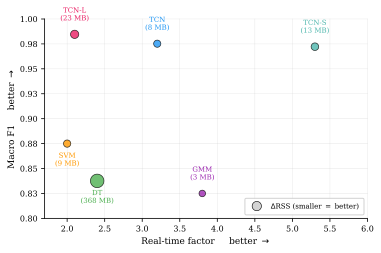
\includegraphics[width=0.85\textwidth]{figures/experiments/cpu_benchmark.pdf}
\caption{Cost vs effectiveness trade-off.}
\label{fig:cpu_benchmark}
\end{figure}

\break

Every model clears the $2\times$ real-time floor at one CPU thread, so the choice between them is on cost rather than streaming feasibility.
TCN-S is the real-time-factor winner, about $40\,\%$ above the next model and $65\,\%$ above the reference TCN.
GMM holds the memory corner, two orders of magnitude less than the decision tree and several times less than any neural model.

\subsection{Symbolic complexity}
\label{subsec:exp_complexity_symbolic_results}

The measured numbers from the previous section are hardware-specific.
This subsection complements them with hardware-independent complexity metrics derived from each model's architecture.

\subsubsection{Reported metrics}

The values come from three sources: the trained models, the streaming inference code, and formulas over each model's architecture.

Parameter counts are read directly from the trained models.
For the TCN family, PyTorch's parameter iterator gives the count.
For the traditional models, the trained scikit-learn estimators expose the relevant sizes: tree node count for the decision tree, support-vector matrix size for SVM, and mixture parameters for GMM.

The number of multiply-accumulate operations (MACs) per output frame follows from how each model is actually run in streaming mode.
The TCN family's backbone is stateless and re-runs over its full receptive-field buffer on every decision, so MACs per frame equal the off-line per-frame cost times the receptive-field length in feature frames.
For the traditional models, MACs per frame count the operations on the active decision path: one comparison per tree-depth level for the decision tree, the kernel evaluation across all support vectors for SVM, or the log-likelihood computation across all mixture components for GMM.
The rolling-decision smoothing adds a small constant on top.

The receptive field for the TCN family follows \Cref{eq:tcn_rf_full} with the per-variant kernel size, blocks per stack, and number of stacks substituted in.
For the traditional models, the receptive field is the feature-extractor window ($300\,\text{ms}$ for the decision tree, $1\,\text{s}$ for GMM and SVM).

\Cref{tab:complexity_symbolic} reports the three resulting columns:
\begin{itemize}
    \item \textbf{Parameter count}: total number of trainable weights.
    \item \textbf{MACs/frame}: multiply-accumulate operations executed to produce one output frame, including the receptive-field re-run that the current streaming implementation performs per decision.
    \item \textbf{Receptive field (RF)}: temporal span of input the model conditions on per decision.
\end{itemize}

\begin{table}[h]
\centering
\small
\begin{tabular}{lrrr}
\toprule
\textbf{Model} & \textbf{params} & \textbf{MACs/frame} & \textbf{RF (ms)} \\
\midrule
\texttt{DT}    & $4.34$\,M & $178$     & $300$ \\
\texttt{GMM}   & $474$     & $216$     & $1000$ \\
\texttt{SVM}   & $521$\,K  & $469$\,K  & $1000$ \\
\texttt{TCN-S} & $4.6$\,K  & $545$\,K  & $2810$ \\
\texttt{TCN}   & $33$\,K   & $11.6$\,M & $8382$ \\
\texttt{TCN-L} & $389$\,K  & $137$\,M  & $8382$ \\
\bottomrule
\end{tabular}
\caption{Symbolic complexity.}
\label{tab:complexity_symbolic}
\end{table}

Streaming MAC count varies by orders of magnitude across the family.
The decision tree and GMM are the cheapest, three to six orders of magnitude below the rest.
The decision tree's count is mostly tree-branch comparisons rather than dense MACs, so the wall-clock benchmark of \Cref{tab:complexity_t1_results} is a more reliable cost ordering at the low end.

Within the TCN family, TCN-S is roughly $21\times$ below the reference TCN in MACs.
The wall-clock reduction is smaller ($1.6\times$ faster), since pipeline overhead does not scale with MAC count.
TCN-L is the most expensive variant, with most of the cost in the LSTM head's persistent-state matrix multiplication.

Receptive fields span an order of magnitude across the family, with TCN-S at roughly one-third of the reference TCN's window.
TCN-S combines that shorter receptive field with halved filter count to reach the $21\times$ MAC reduction at only $0.003$ macro F1 score loss, so the reduced capacity suffices for most of the test distribution.

\subsubsection{Parameter vs compute}
\Cref{fig:complexity_symbolic} plots parameter count against streaming MACs per output frame on log-log axes to visualize how the two cost dimensions decouple across the family.

\begin{figure}[h]
\centering

\includegraphics[width=0.85\textwidth]{figures/experiments/symbolic_complexity.pdf}
\caption{Parameter count against streaming MACs (log-log).}
\label{fig:complexity_symbolic}
\end{figure}

\break

The decision tree sits in the high-parameter, low-compute corner (large tree, comparison-only inference).
The TCN family occupies the low-parameter, high-compute corner (small weight tensors with a receptive-field re-run on every decision).
GMM and SVM bridge the two diagonals.

\subsection{Critical subset check}
\label{subsec:exp_critical_results}

The critical subset (\Cref{sec:dataset_critical_subset}) was built towards the end of work on this thesis to sanity-check the models through manual review rather than through aggregate numbers alone.
Predictions are plotted over a hand-labeled ground truth.
The sanity-check pair, the misclassified-background clip, and the extreme-music clip show all six classifiers.
The remaining figures show TCN-S alone, the proposed method of this thesis.
Each figure below shows $15\,\text{s}$ of one representative clip.
The rest of the subset followed the same trajectory: every remaining clip either worked as expected, or failed with the same \emph{Background}-mistaken-for-\emph{Music} pattern shown in \Cref{fig:crit_unknown_noise}.
This subsection summarizes the findings.

\break

\Cref{fig:crit_sanity} shows every model classifying a $15\,\text{s}$ pop-music clip and a clean-speech recording.

\begin{figure}[h]
    \centering
    
\includegraphics[width=\textwidth]{figures/critical/music_sanity.pdf}
    
\includegraphics[width=\textwidth]{figures/critical/speech_sanity.pdf}
    \caption{Classifier decisions on a pop music clip (top) and a clean speech recording (bottom).}
    \label{fig:crit_sanity}
\end{figure}

Every model classifies both clips almost perfectly.
The decision tree misclassifies one frame on the pop clip, and the SVM scatters a few frames on speech.
The decision tree's output also flickers more than the others, traced to its $10\,\text{ms}$ frame length (further discussed in \Cref{sec:conclusion_limitations}).

\bigskip

The next two figures each pair a \emph{Background} clip with the same clip mixed with \emph{Speech}.

\begin{figure}[h]
    \centering
    
\includegraphics[width=\textwidth]{figures/critical/noise_good_bird.pdf}
    
\includegraphics[width=\textwidth]{figures/critical/speech_noise_good_bird.pdf}
    \caption{TCN-S on a correctly classified \emph{Background} clip (top) and the same clip with \emph{Speech} overlaid (bottom).}
    \label{fig:crit_known_noise}
\end{figure}

\Cref{fig:crit_known_noise} is the expected case and slightly exceeds expectations.
When TCN-S labels the noise as \emph{Background} on its own, it also recognizes \emph{Speech} mixed over the same noise at $-3\,\text{dB}$ SNR.

\begin{figure}[h]
    \centering
    
\includegraphics[width=\textwidth]{figures/critical/noise_bad_fan.pdf}
    
\includegraphics[width=\textwidth]{figures/critical/speech_noise_bad_fan.pdf}
    \caption{Misclassified \emph{Background} clip across all six classifiers (top) and the same clip with \emph{Speech} overlaid on TCN-S (bottom).}
    \label{fig:crit_unknown_noise}
\end{figure}

\break

\Cref{fig:crit_unknown_noise} is the opposite case.
Every classifier labels the unknown background as \emph{Music}, and TCN-S sticks to \emph{Music} even when speech enters the mix.
This is the largest negative finding of the review: the dataset's \emph{Background} class under-represents the variety of ambient sound a real deployment encounters.
The remedy is discussed in \Cref{sec:conclusion_limitations}.

\bigskip

\Cref{fig:crit_music_speedcore} shows classifier decisions on a $400\,\text{BPM}$ electronic clip.

\begin{figure}[h]
    \centering
    
\includegraphics[width=\textwidth]{figures/critical/speedcore.pdf}
    \caption{Classification decisions on extreme music.}
    \label{fig:crit_music_speedcore}
\end{figure}

Manual review of this and other extreme-music recordings (Belgian jumpup, beatbox) was almost perfect, a positive surprise.

\break

\Cref{fig:crit_som_ms_msom} groups speech over music, multi-speaker recordings, and multi-speaker over music.

\begin{figure}[h]
    \centering
    
\includegraphics[width=\textwidth]{figures/critical/speech_over_music.pdf}\\[4pt]
    
\includegraphics[width=\textwidth]{figures/critical/multispeaker.pdf}\\[4pt]
    
\includegraphics[width=\textwidth]{figures/critical/multispeaker_over_music.pdf}
    \caption{TCN-S decisions on speech over music (top), multi-speaker recording (middle), and multi-speaker over music (bottom).}
    \label{fig:crit_som_ms_msom}
\end{figure}


\Cref{fig:crit_som_ms_msom} reveals a second coverage limitation.
TCN-S handles speech over music (top) with brief flicker at transitions.
Multi-speaker speech alone (middle) already strains it.
Adding music on top of multi-speaker speech (bottom) overwhelms the model entirely.

\bigskip

The walk-through served its sanity-check purpose: every model classifies the content it was capable of handling as expected.
It also uncovered a dataset gap: when a classifier cannot handle an ambient sound, it labels the clip as \emph{Music}, and TCN-S keeps that label even when speech enters the mix.
Expanding the dataset's \emph{Background} coverage is taken up as future work in \Cref{sec:conclusion_future}.

